\chapter{Object reconstruction and event simulation}
\chaptermark{Object reconstruction and event simulation}  
\thispagestyle{plain}  % First page has default style
\pagestyle{chapterpages}
\label{Section:Chapter4}
\minitoc

This chapter presents the reconstruction and identification of physics objects in the CMS detector, which is foundational to all analyses performed in this thesis. In particular, $\PGt$ lepton reconstruction is a central focus. This is a particularly challenging task due to its short lifetime and complex decay modes, which can involve a mix of charged and neutral hadrons, electrons, muons, and undetectable neutrinos. Therefore, excellent performance of multiple reconstruction components is required, including charged-particle tracking, electromagnetic and hadronic calorimetry, muon identification, and displaced secondary vertexing.

However, operating in a high-multiplicity environment introduces additional challenges for reconstructing and identifying physics objects. There is no guarantee that a reconstructed particle corresponds to a genuine physics object; such cases are referred to as \textit{misidentified} or \textit{``fake'' objects}. For example, jets initiated by quarks or gluons can sometimes be misidentified as hadronic $\PGt$ decays; leptons originating from heavy-flavour decays within jets may mimic prompt electrons or muons; and, conversely, muons and electrons can occasionally be misidentified as jets. To mitigate these effects, object identification algorithms incorporate \textit{multivariate discriminants} and \textit{\acp{WP}} that are tuned to balance efficiency and misidentification rates. However, in some cases, these strategies only partially suppress such backgrounds.

A more complete and accurate event description is achieved by correlating information from all layers of the CMS detector to reconstruct and identify individual particles. This integrated methodology is known as \textbf{\ac{PF}} reconstruction. The implementation of this approach within CMS is detailed in this chapter.

In addition to reconstruction, this chapter also outlines the simulation of proton-proton collision events used to model both signal and background processes. Particular attention is given to the simulation of backgrounds relevant to final states with two or more $\PGt$ leptons, as encountered in the analyses described in this thesis.

\section{Reconstruction of Particle Flow detector elements}
\label{Section:Chapter4_Reconstruction_of_PF_elements}
\subsection{Track reconstruction}
The first stage of the reconstruction process, known as \textbf{local reconstruction}~\cite{CMS_TrackerPerformance_2014,CMS_Track_Reconstruction_Run2_3}, uses \textit{clusters}. These are groups of adjacent strips with signals above predefined thresholds, identified during \ac{FED} readout, and are used to reconstruct particle hits in the silicon tracker. For each cluster, both the position and its associated uncertainty are estimated within a local coordinate system defined by the sensor geometry. These locally reconstructed hits form the basis for the subsequent \textbf{global reconstruction}~\cite{CMS_TrackerPerformance_2014,CMS_Track_Reconstruction_Run2_3} of particle trajectories.

Global track reconstruction is facilitated by the \textbf{\ac{CTF}} algorithm~\cite{CMS_TrackerPerformance_2014,CMS_Track_Reconstruction_Run2_3}, an adaptation of the combinatorial \textit{\ac{KF}}~\cite{KF_1,KF_2,KF_3}\footnote{KF~\cite{KF_4} is recursive algorithm that uses a series of measurements over time to estimate the state of a system. This is done by estimating a joint probability distribution over the variables of interest at each time step.} approach. This adaptation enables pattern recognition and track fitting to be performed within a unified framework, allowing hits to be incrementally added and track parameters to be continuously updated in a process known as \textbf{iterative tracking}. A single iteration of the CTF algorithm proceeds in four steps:

\begin{enumerate}
    \item \textbf{Seed generation}: Initial track candidates are formed using a small number of hits (typically two or three) in the innermost layers of the tracker. Each \textit{seed} provides an initial estimate of the particle's trajectory parameters, such as position, direction, and momentum, as well as their associated uncertainties. 
    \item \textbf{Track finding}: Seed trajectories are extrapolated along the expected trajectory of a charged particle using a Kalman Filter (KF). At each detector layer, additional hits along the expected flight path are identified and associated with the track candidate; the trajectory parameters are then updated accordingly. This process is repeated iteratively until the outermost layer of the detector is reached, gradually building complete track candidates from the initial seeds.
    \item \textbf{Track fitting}: The final trajectory is refitted iteratively to improve the estimate of the track parameters. This is done using a combination of a KF and a smoother, incorporating all available hit information.
    \item \textbf{Track selection}: Tracks are required to pass a set of quality flags.
\end{enumerate}

The \textbf{iterative tracking} procedure in CMS is performed in successive iterations, each designed to target different classes of tracks, as summarised in Table~\ref{Table:Chapter4_IterativeTrackingSeeds}. The initial iterations target tracks that are the easiest to find (\eg high $p_\mathrm{T}$ tracks, and tracks produced near the primary interaction point). After each iteration, the combinatorial complexity is reduced by removing hits associated with tracks. This enables later iterations to target more challenging classes of tracks (\eg low $p_\mathrm{T}$ tracks, and tracks displaced from the interaction point). 

\begin{table}[h]
\centering
\renewcommand{\arraystretch}{1.5} % Increase row height
\arrayrulecolor{black} % Ensure outer borders are black
\begin{tabular}{|c|l|l|l|}
\hline
Iteration & Name & Seeding & Targeted Tracks \\ \hline \hline
1         & InitialStep              & pixel quadruplets           & prompt, high $p_\mathrm{T}$    \\
\arrayrulecolor{lightgray} \hline
2         & LowPtQuad                & pixel quadruplets           & prompt, low $p_\mathrm{T}$    \\
\arrayrulecolor{lightgray} \hline
3         & HighPtTriplet            & pixel triplets             & prompt, hight $p_\mathrm{T}$                \\
\arrayrulecolor{lightgray} \hline
4         & LowPtTriplet             & pixel triplets             & prompt, low $p_\mathrm{T}$                \\
\arrayrulecolor{lightgray} \hline
5         & DetachedQuad             & pixel quadruplets          & b hadron decays, R $\leq 5\unit{cm}$      \\
\arrayrulecolor{lightgray} \hline
6         & DetachedTriplet          & pixel triplets              & b hadron decays, R $\leq 10\unit{cm}$      \\
\arrayrulecolor{lightgray} \hline
7         & MixedTriplet             & pixel+strip triplets        & displaced, R $\leq 7\unit{cm}$                \\
\arrayrulecolor{lightgray} \hline
8         & PixelLess                & strip triplets/pairs        & very displaced, R $\leq 25\unit{cm}$          \\
\arrayrulecolor{lightgray} \hline
9         & TobTec                   & strip triplets/pairs        & very displaced, R $\leq 60\unit{cm}$          \\
\arrayrulecolor{lightgray} \hline
10         & JetCoreRegional          & pixel+strip pairs          & inside high $p_\mathrm{T}$ jets                 \\
\arrayrulecolor{lightgray} \hline
11         & MuonSeededInOut         & muon-tagged tracks          & muons                               \\
\arrayrulecolor{lightgray} \hline
12        & MuonSeededOutIn          & muon detectors              & muons                               \\
\arrayrulecolor{black} \hline
\end{tabular}
\caption[Summary of iterative tracking steps in CMS]{Summary of the iterations used in the CMS iterative tracking algorithm. Table taken from Ref.~\cite{ParticleFlow,LocalReconstructionSteps}.}
\label{Table:Chapter4_IterativeTrackingSeeds}
\end{table}

\subsection{Vertex reconstruction}

The primary goal of the CMS vertex reconstruction~\cite{CMS_TrackerPerformance_2014} is to determine the positions and associated uncertainties of all pp interaction vertices in an event, including both the \textbf{\ac{PV}} (associated with the \textit{``signal'' interaction}) and any additional vertices originating from PU collisions, using all available reconstructed tracks. The reconstruction process is performed in three main steps: 

\begin{enumerate}
    \item \textbf{Track selection}: Tracks consistent with originating promptly near the centre of the luminous region (referred to as the beam spot) are selected. This selection is based on applying quality requirements to the tracks, such as cuts on the transverse impact parameter\footnote{The impact parameter is defined as the distance of closest approach of a charged particle’s trajectory to the PV} significance relative to the beam spot and minimum numbers of associated pixel and strip hits.
    \item \textbf{Track clustering}: Tracks are clustered into groups that appear to be originating from the same vertex. This clustering is performed based on their z-coordinate at the point of closest approach to the beam spot using a \textit{deterministic annealing algorithm}~\cite{DeterministicAnnealing}.
    \item \textbf{Vertex fitting}: Candidate vertices composed of at least two tracks are fitted using an \textit{adaptive vertex fitter}~\cite{VertexFitting_2006,VertexFitting_2007} to determine the best estimate of the vertex parameters. These parameters include the $x$, $y$, and $z$ positions, the associated covariance matrix, and indicators of fit quality. Additionally, the adaptive fit assigns a weight between 0 and 1 to each track, reflecting the probability that the track is genuinely associated with the vertex.
\end{enumerate}

Once all the vertices are reconstructed, a collection is formed, which is ordered by the quadratic sum of the transverse track momenta associated with each vertex, $\sum_{\text{tracks}} p_{\mathrm{T}}^2$. The vertex with the largest sum is assumed to most likely correspond to the vertex of the hard scattering process~\cite{ParticleFlow}. The efficiency to correctly identify the PV when at least three tracks are associated is close to 100\%~\cite{CMS_TrackerPerformance_2014}. The resolution of the PV position, particularly in the $x$ and $z$ coordinates, has been measured using $\sqrt{s} = 13\ \mathrm{TeV}$ collision data~\cite{PrimaryVertex_Resolution} and is found to improve rapidly as the summed $p_{\mathrm{T}}$ of the associated tracks increases, as shown in Fig.~\ref{Figure:Chapter4_PrimaryVertex_Resolution}.

\begin{figure}[h]
    \centering
    % First row
    \begin{subfigure}[b]{0.49\textwidth}
        \centering
        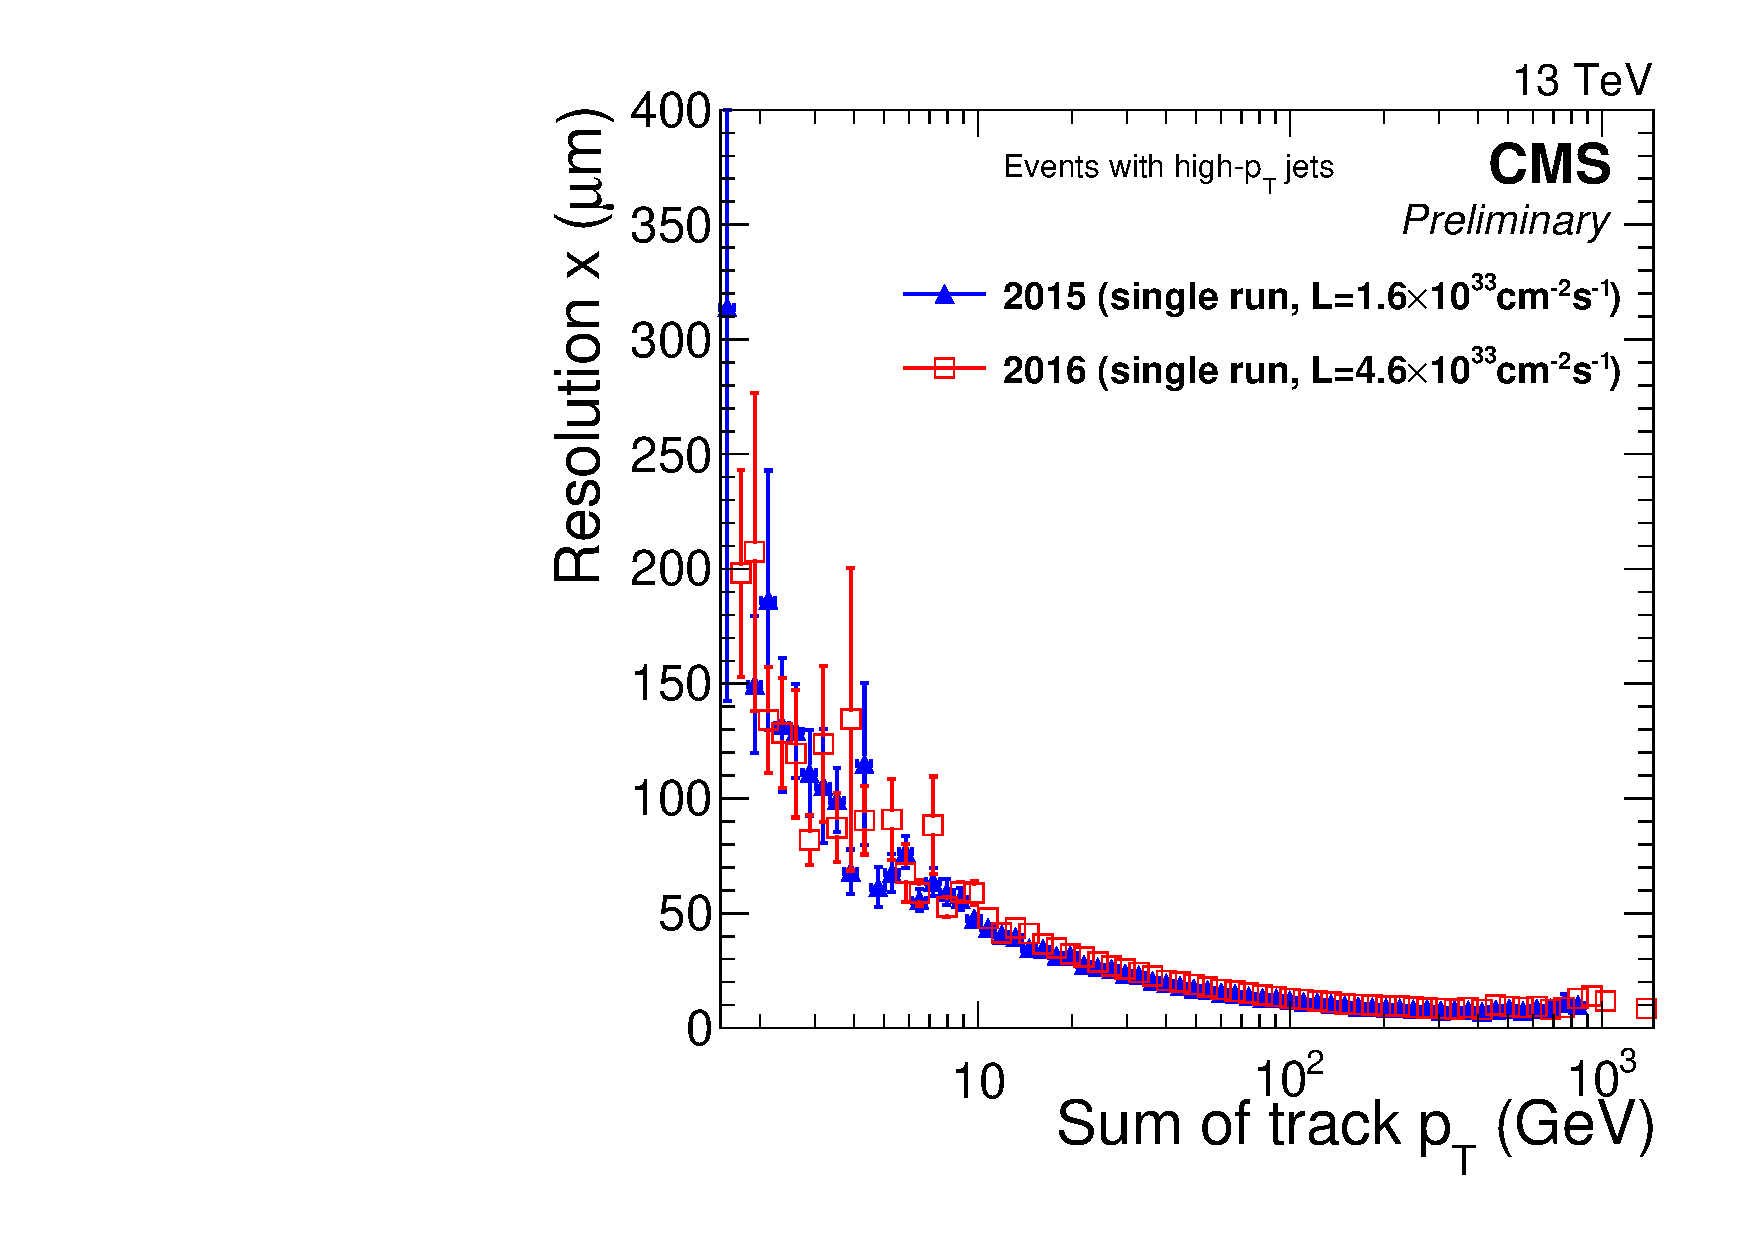
\includegraphics[width=\textwidth]{Figures/Chapter4/resolution_sumpt_x.pdf}
        \caption{}
    \end{subfigure}
    \begin{subfigure}[b]{0.49\textwidth}
        \centering
        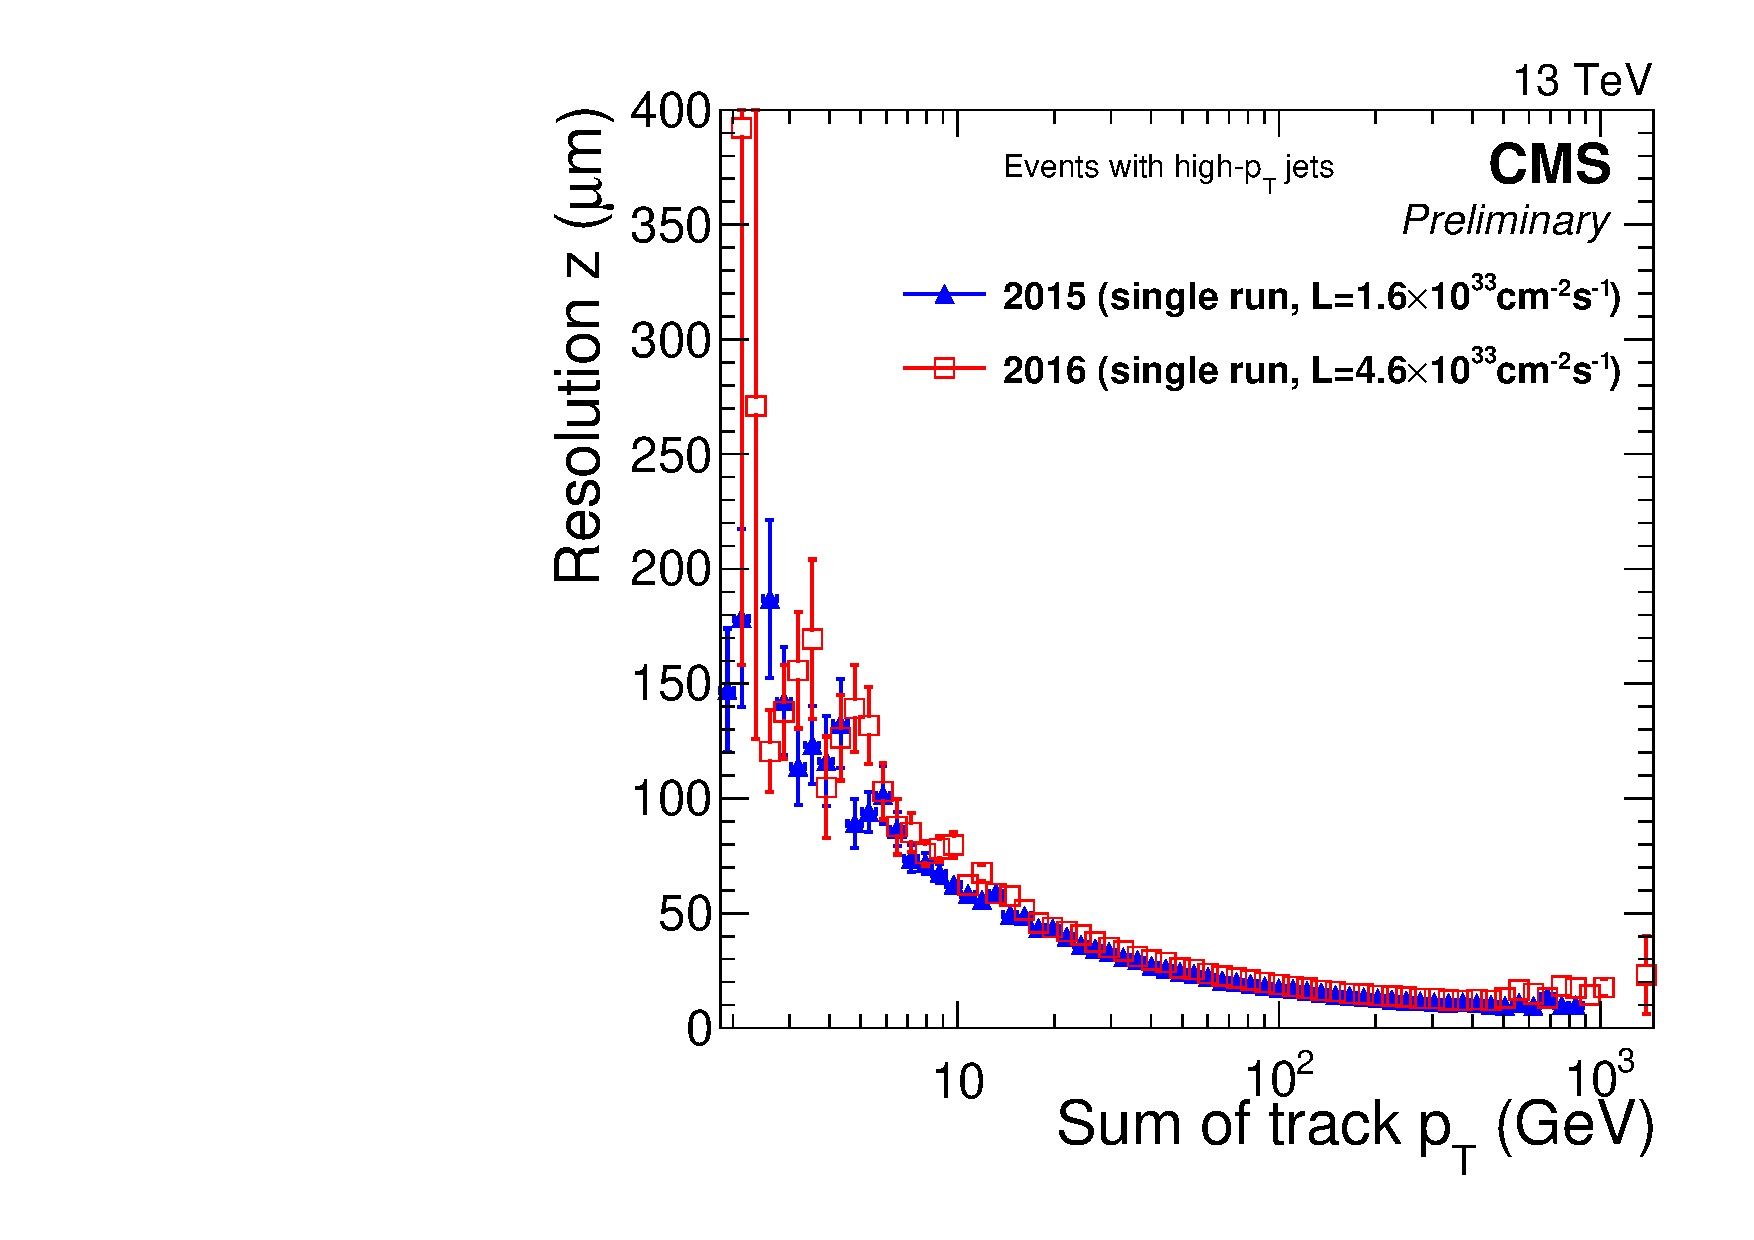
\includegraphics[width=\textwidth]{Figures/Chapter4/resolution_sumpt_z.pdf}
        \caption{}
    \end{subfigure}
\caption[Resolution of the reconstructed transverse and longitudinal positions of the primary vertex using CMS collision data (2015 \& 2016)]{Resolution of the reconstructed PV position in the \textbf{(a)} transverse ($x$) and \textbf{(b)} longitudinal ($z$) directions as a function of the $\sum p_\mathrm{T}$ of the associated tracks. Measurements are shown for pp collisions recorded in 2015 (blue) and 2016 (red). Figures taken from Ref.~\cite{PrimaryVertex_Resolution}.}

\label{Figure:Chapter4_PrimaryVertex_Resolution}
\end{figure}

\subsection{Electron tracking}
\label{Section:Chapter4_ElectronTracking}
Electron reconstruction in CMS leverages both tracking information from the silicon tracker and energy deposits in the ECAL. Two complementary seeding strategies are employed: one utilising energetic ECAL clusters ($E_\mathrm{T} > 4\GeV$), referred to as the \textit{ECAL-based approach}, and the other utilising reconstructed tracks, referred to as the \textit{tracker-based approach}.

As electrons traverse the CMS tracker, they emit a sizeable fraction of their energy as bremsstrahlung photons due to the significant material thickness (see Fig.~\ref{Figure:Chapter3_Tracker_MaterialBudget}). The performance of the \textbf{ECAL-based approach} therefore depends on the ability to recover this radiated energy while minimising contamination from nearby particles. These photons are predominantly emitted along the electron’s direction but become laterally displaced in $\phi$ due to the curvature of the track in the magnetic field. To capture this energy, a \textit{supercluster} is constructed by merging multiple ECAL clusters within a narrow $\eta$ window and an extended $\phi$ window around the expected electron trajectory~\cite{ParticleFlow}. However, this method exhibits significant inefficiencies in high-density environments, such as when electrons are embedded in jets, where overlapping energy deposits from nearby particles can bias the supercluster’s energy and position. It also suffers when back-propagating from the supercluster to the interaction point, as the supercluster may be compatible with multiple hits from other charged particles, increasing the risk of misreconstruction. Further inefficiencies arise for low-$p_\mathrm{T}$ electrons, where the radiated energy is spread over a broad $\phi$ range, preventing complete energy recovery within a single supercluster.

To recover electrons missed by the ECAL-based method, the \textbf{tracker-based} approach is employed. This approach leverages the high efficiency of the iterative tracking algorithm, which can reliably reconstruct both non-radiating and radiating electrons. Tracks with $p_\mathrm{T} > 2\GeV$ from iterative tracking are considered as potential electron seeds. When bremsstrahlung emission is minimal, the corresponding track can be well reconstructed, as indicated by a well-behaved $\chi^2$ from the track fit\footnote{The chi-squared ($\chi^2$) statistic quantifies the agreement between the measured hit positions and the predicted trajectory of the track. A low $\chi^2$ indicates a good-quality fit and, therefore, a well-reconstructed track.}, and propagated safely to the ECAL inner surface for matching with the nearest ECAL cluster. However, when bremsstrahlung is more significant, the pattern recognition may still recover the track, but often with degraded fit quality (\ie fewer associated hits or a larger $\chi^2$). To address this, a preselection is applied based on the number of hits and the $\chi^2$ of the initial fit, after which tracks are refitted using a \ac{GSF} algorithm~\cite{GSF_Algorithm}. Unlike the KF used in standard tracking, the GSF is specifically designed to accommodate the sudden and substantial energy losses along the trajectory.

\subsection{Muon tracking}

Muon reconstruction~\cite{ParticleFlow} in CMS combines information from the dedicated muon detection system with precision tracking from the inner tracker. Three complementary reconstruction strategies are employed, leading to different possible definitions for reconstructed muons:

\begin{itemize}
    \item \textbf{Standalone muon}: In the muon system, hits from each DT or CSC are clustered into track segments, which serve as seeds for pattern recognition. These seeds are used to collect compatible hits across all muon subsystems (DT, CSC, RPC) to reconstruct the muon trajectory. This is referred to as a standalone muon track because the reconstruction is performed using only information from the muon system.
    \item \textbf{Global muon}: Standalone muon tracks are matched to tracks in the inner tracker. If there is a compatible match, a combined fit of the hits from the inner tracker and muon system is performed to form a global muon track.
    \item \textbf{Tracker muon}: Inner tracks with sufficient transverse ($> 0.5\GeV$) and total momenta ($>2.5\GeV$) are extrapolated to the muon system and classified as tracker muons if they are spatially compatible with at least one muon segment.
\end{itemize}

\textit{Global muon reconstruction} is most efficient for muons that traverse multiple muon detector planes. However, at low momenta ($<10\GeV$), larger multiple scattering in the steel return yoke reduces the efficiency of global muon reconstruction, as it becomes more difficult to associate segments in multiple muon stations. In such cases, \textit{tracker muon reconstruction} is more efficient, as it requires only a single matched segment~\cite{CMS_Muon_System_Performance_2}. The high efficiency of both the inner tracker and muon segment reconstruction ensures that approximately 99\% of muons within the detector's acceptance are reconstructed as either global or tracker muons, and often as both.  In such cases, global and tracker muons sharing the same inner track are merged into a single muon candidate.

\subsection{Calorimeter clusters}

The reconstruction of calorimeter-based PF elements in CMS is designed to~\cite{ParticleFlow}:

\begin{itemize}
    \item Identify and measure the energy and direction of stable neutral particles
    \item Distinguish neutral particle energy deposits from those of charged hadrons
    \item Reconstruct electrons along with their associated bremsstrahlung photon energy deposits
    \item Aid the energy measurement of charged hadrons in cases where the track information is imprecise
\end{itemize}

A dedicated clustering algorithm~\cite{ParticleFlow} is applied separately in each calorimeter subsystem, including the barrel and endcap regions of the ECAL and HCAL, as well as the ECAL preshower. For the HF subdetector, clustering is not performed; instead, each cell directly forms an electromagnetic or hadronic cluster. 

\textit{Cluster seeds} are identified in the first step of the algorithm. These are calorimeter cells with energy above a specified threshold that also represent local maxima with respect to their neighbouring cells. In the second step, \textit{topological clusters} are grown from the seeds by adding neighbouring cells that share at least a corner with an existing cluster cell and have energy above a threshold, typically set to twice the noise level. In the final step, an expectation-maximisation algorithm based on a Gaussian mixture model is applied to decompose each topological cluster into one or more individual \textit{``PF'' clusters}.

\section{Particle Flow}
The tracking information and calorimeter clusters described in Section~\ref{Section:Chapter4_Reconstruction_of_PF_elements} form the foundational inputs to the \textit{PF algorithm}. As a single particle generally produces multiple PF elements across the various CMS subdetectors, the reconstruction process begins with a \textit{link algorithm} that connects these elements. The primary limitation of the PF algorithm lies in its dependence on accurately linking detector elements that originate from the same particle. As such, its performance is sensitive to the granularity of the subdetectors, the local density of particles in the event, and the amount of material a particle traverses before reaching the calorimeters and the muon system.

The \textit{linking procedure} begins by evaluating nearby pairs of elements in the $\eta$–$\phi$ plane and, where applicable, defines a distance parameter to quantify the quality of the link. Links between tracks in the central tracker and calorimeter clusters are established by extrapolating a track from its last measured hit in the tracker to different depths in the ECAL (at the expected electron shower maximum) and HCAL (at a depth of one interaction length). A link is created if the extrapolated position falls within the boundaries of the cluster. Similarly, a track-cluster distance parameter is defined as the distance between the extrapolated track position and the cluster position in $\eta$–$\phi$ plane. When multiple HCAL clusters are linked to the same track, or several tracks are associated with the same ECAL cluster, this distance parameter is used to resolve ambiguities by retaining only the link with the smallest value. To recover energy lost via electron bremsstrahlung, tangents to the GSF tracks are extrapolated to the ECAL and used to link clusters within a narrow $\eta$ window ($\Delta\eta < 0.05$), while converted photons are recovered by linking track pairs using a dedicated conversion finder~\cite{DedicatedConversionFinder}. In addition, links between calorimeter clusters (HCAL-ECAL \& ECAL-PS) are established based on their positions in the more granular calorimeter. Similarly, a cluster-cluster distance parameter is defined as the distance between the cluster positions in the $\eta-\phi$ plane. As in the case of track–cluster associations, when multiple clusters are compatible, only the link with the smallest distance is retained. Finally, links between tracks in the central tracker and information in the muon system are established through a global fit, with the distance parameter defined as the $\chi^2$ of the fit. In cases where multiple associations are possible, only the link with the lowest $\chi^2$ is retained to ensure the most compatible match.

Once all valid links are established, groups of interconnected elements, either through direct or indirect links, are assembled into \textit{PF blocks}. Each PF block is processed by the PF algorithm, which operates on the block following a well-defined sequence of steps to reconstruct and identify a set of particles. The procedure is as follows:

\begin{enumerate}
    \item \textbf{PF muons}: Global muons present within the block are identified as PF muons if their associated track is consistent with minimal energy deposition in the calorimeters. Once identified, the corresponding tracker and muon elements are removed from the block.
    \item \textbf{PF electrons}: Tracks not previously identified as muons are submitted to a pre-identification step that selects candidate electrons based on characteristic bremsstrahlung patterns observed in the tracker. As described in Section~\ref{Section:Chapter4_ElectronTracking}, these candidates are refitted with a Gaussian Sum Filter (GSF), and a multivariate discriminant combining tracking and ECAL variables is applied. If the candidate passes the discriminant, it is identified as a PF electron, and the associated track and ECAL clusters are removed from the block.
    \item \textbf{PF charged hadrons}: Remaining tracks give rise to PF charged hadrons. Associated tracks and calorimeter clusters are removed from the block.
    \item \textbf{PF photons \& PF neutral hadrons}: Non-compatible calorimeter clusters with track momentum are interpreted as neutral particles, following:
    \begin{enumerate}
        \item Depending on the relative energy in each calorimeter, both a PF photon (from ECAL) and a PF neutral hadron (from HCAL) may be created to account for the excess.
        \item If the excess energy is primarily in the ECAL and exhibits electromagnetic shower characteristics, only a PF photon is created.
        \item Remaining ECAL and HCAL clusters with no associated tracks are interpreted as PF photons and PF neutral hadrons, respectively.
    \end{enumerate}
\end{enumerate}

\section{Object identification}
\label{Section:Chapter4_Object_Identification}

The final output of the PF algorithm is a list of reconstructed particles, referred to as \textit{PF candidates}. However, PF does not inherently guarantee that the candidates correspond to genuine prompt physics objects. Therefore, dedicated identification (ID) algorithms are required to translate these PF candidates into physics objects suitable for analysis. This section serves to describe the object identification strategies used in this thesis.

\subsection{Electrons}
\label{Section:Electron_Identification}

Electrons are identified using a \ac{MVA} approach, where a \ac{BDT} algorithm~\cite{Electron_ID} is employed to distinguish genuine prompt electrons from backgrounds. These backgrounds include electrons from photon conversions, misidentified hadrons, and non-prompt electrons from the decay of hadrons. The set of discriminating variables used by the BDT can be grouped into the following categories:

\begin{itemize}
    \item \textbf{Track-cluster matching observables}: These variables compare measurements obtained from the ECAL and the tracker, including both geometrical matching between the ECAL supercluster and the tracker, as well as energy-momentum matching.
    \item \textbf{Calorimetric observables}: These variables are purely calorimetric and are used to improve the separation between genuine and misidentified electrons. One example is the transverse shape of EM showers in the ECAL, where the typically narrow profile of EM showers is exploited in contrast to the broader shape of hadronic showers. Additional calorimetric observables include the hadronic-to-electromagnetic energy ratio ($H/E$), which is expected to be small for electrons, and the energy deposited in the HCAL and preshower (in the endcaps), which further helps to discriminate against hadronic backgrounds.
    \item \textbf{Tracking observables}: These variables are used to enhance discrimination between electrons and charged hadrons by leveraging detailed information from the GSF track fit, as well as discrepancies between the GSF and KF track reconstructions.
\end{itemize}

A working point corresponding to 90\% signal efficiency is used in this thesis, meaning that approximately 90\% of genuine prompt electrons are correctly identified~\cite{ElectronID_Performance}. To accommodate different analysis needs, two versions of the BDT discriminator are employed: one that includes isolation variables during training, and one that does not, allowing flexibility in environments with varying levels of surrounding activity. 

In addition to the BDT-based electron identification, isolation requirements are essential for further suppressing backgrounds from misidentified jets or genuine electrons within jets arising from heavy-flavour decays. These background electrons are typically accompanied by significant nearby energy deposits, which can be effectively rejected by imposing an isolation criterion. A simple isolation variable is based on detector-based isolation. This approach computes the scalar sum of transverse energy deposits in the ECAL or HCAL, or the scalar sum of the $p_\mathrm{T}$ of tracks originating from the primary collision vertex, within a cone of radius $\Delta R$ (typically 0.3 or 0.4) around the electron direction. 

A more refined isolation variable is the \textit{PF isolation} ($I_{\text{PF}}^e$)~\cite{ElectronID_Performance}, which utilises PF candidates reconstructed within a cone around the electron's direction:

\begin{equation_pad}
    I_{\text{PF}}^e = \frac{1}{p_\mathrm{T}^e} \left( \sum_{\text{h}^{\pm}} p_\mathrm{T} + \text{max} \left[0, \sum_{\text{h}^{0}} p_\mathrm{T} + \sum_{\gamma} p_\mathrm{T} - \rho A_{\text{eff}}\right]  \right)
\label{Equation:Chapter4_PFIso_Electron}
\end{equation_pad}

where the sums include all PF charged hadrons ($h^\pm$) originating from the primary vertex, neutral hadrons ($h^0$), and photons ($\gamma$). The term $\rho A_{\text{eff}}$ accounts for the contribution from PU interactions.

\subsection{Muons}
\label{Section:Muon_Identification}
As with electrons, a dedicated identification strategy is employed to distinguish genuine prompt muons originating from the PV from non-prompt muons produced in hadron decays, as well as from charged hadrons misidentified as muons. In this thesis, a \textit{cut-based} muon identification approach is used, specifically adopting the \textit{medium WP}. The criteria of this WP are as follows:

\begin{itemize}
    \item The muon must be identified by PF, which requires it to be reconstructed as either a tracker or global muon.
    \item Track must be reconstructed with hits in at least 80\% of the inner tracker layers along its path.
    \item Muon segment compatibility of tracker-only muons must be greater than 0.451\footnote{Muon segment compatibility~\cite{CMS_Muon_System_Performance} is computed by propagating the tracker track to the muon system and evaluating both the number of matched segments across stations and the closeness of the matches in position and direction. The variable ranges from 0 to 1, with higher values indicating better compatibility with a genuine muon.}.
    \item For muons reconstructed as both tracker and global muons, the following criteria must be satisfied:
    \begin{enumerate}
        \item Muon segment compatibility must be greater than 0.303.
        \item The global track fit must have a reduced $\chi^2$ value below 3.
        \item The $\chi^2$ of the position match between tracker muon and standalone muon must be less than 12.
        \item The maximum $\chi^2$ value computed by the kink-finding algorithm\footnote{The kink-finding algorithm evaluates the consistency of the tracker track by splitting it into two separate tracks at multiple points along its trajectory. The resulting segments are compared, and a $\chi^2$ value is assigned to quantify their compatibility with originating from the same continuous track.} must be less than 20.
    \end{enumerate}
\end{itemize}

Isolation requirements are also applied to reduce backgrounds from non-prompt muons, such as those produced in weak decays of hadrons within jets. Similar to electrons, isolation can be defined using PF candidates. The PF relative isolation~\cite{ParticleFlow} is given by:

\begin{equation_pad}
    I_{\text{PF}}^\mu = \frac{1}{p_\mathrm{T}^\mu} \left( \sum_{\text{h}^{\pm}} p_\mathrm{T} + \text{max} \left[0, \sum_{\text{h}^{0}} p_\mathrm{T} + \sum_{\gamma} p_\mathrm{T} - \Delta \beta \sum_{\text{h}^{\pm}\text{,PU}} p_\mathrm{T} \right]  \right)
\end{equation_pad}

where the expression follows the same structure as the PF isolation for electrons (Eq.~\ref{Equation:Chapter4_PFIso_Electron}). The sums run over PF charged hadrons ($h^\pm$) associated with the PV, neutral hadrons ($h^0$), and photons ($\gamma$), all within a cone of radius $\Delta R < 0.4$ around the muon direction. The pileup correction term includes the scalar sum of transverse momenta of charged hadrons not associated with the PV, scaled by a factor $\Delta \beta = 0.5$. This factor corresponds approximately to the ratio of neutral to charged hadron particle production in the hadronisation process of inelastic pp collisions.

\subsection{Jets}
\label{Section:Chapter4_Jets}
While electrons and muons are reconstructed on a per-particle basis, hadronic final states give rise to collimated sprays of particles originating from the fragmentation and hadronisation of quarks and gluons, which must be clustered to form jets. In CMS, jet reconstruction is performed using sequential jet clustering algorithms~\cite{Jet_Algorithm_Performance,Jet_Reconstruction_Run2_Run3}. In this thesis, the anti-$k_\mathrm{T}$ algorithm~\cite{anti_kT} is employed to cluster PF candidates, as implemented in the \textsc{FastJet} package~\cite{FastJet}. This algorithm is selected based on two key criteria: infrared and collinear safety.

This algorithm iteratively groups particles together based on a distance metric ($d_{ij}$), defined as the distance between two objects $i$ and $j$. An additional distance metric, $d_{iB}$, quantifies the distance between object $i$ and the beam axis. The clustering proceeds by identifying the pair $(i,j)$ with the smallest distance. If the minimum corresponds to $d_{ij}$, the objects $i$ and $j$ are merged; if it corresponds to $d_{iB}$, the object $i$ is deemed a final jet and removed from the clustering sequence. This procedure is repeated until no objects remain to be clustered. The distance metrics used by the anti-$k_\mathrm{T}$ algorithm are defined as follows: 

\begin{equation_pad}
    \begin{aligned}
        d_{ij} &= \min\left(p_{\mathrm{T},i}^{-2},\, p_{\mathrm{T},j}^{-2}\right) \frac{\Delta R_{ij}^2}{R^2} \,, \\
        d_{iB} &= p_{\mathrm{T},i}^{-2} \,,
    \end{aligned}
\end{equation_pad}

where $\Delta R_{ij}$ is the distance between objects $i$ and $j$ in the $\eta$–$\phi$ plane, and $R$ is the jet radius parameter, typically set to 0.4. Jets reconstructed with this cone size using the anti-$k_\mathrm{T}$ algorithm are referred to as AK4 jets.

\subsubsection{Pileup mitigation}

One significant constraint to jet clustering in CMS arises from PU. These secondary interactions introduce extra particles that can be clustered into jets, contaminating the jet energy and degrading both the resolution and substructure observables. To mitigate this, CMS employs dedicated PU mitigation strategies~\cite{PU_Mitigation}. The standard method in Run 2 was the \textbf{\ac{CHS}} algorithm~\cite{ParticleFlow}, which leverages information from the tracker to remove charged hadrons that are not associated with the PV before jet clustering. Although CHS substantially improves jet energy resolution, its reliance on post-clustering corrections~\cite{JetEnergyCalibration} on the four-momenta limits its ability to preserve jet shape and subtracture. To overcome this limitation, an alternative approach known as \textbf{\ac{PUPPI}}~\cite{PUPPI} has been developed. PUPPI computes on an event-by-event basis a weight for each particle. This weight quantifies the likelihood of the particle originating from the PV, and it is used to scale the particle momenta before clustering. Therefore, allowing jet reconstruction to be less sensitive to PU effects. Both CHS and PUPPI are employed in this thesis: CHS-based jets are used in Chapter~\ref{Section:Chapter_4tau}, while PUPPI-based jets are used in Chapter~\ref{Section:Chapter_CP}. A schematic comparison of the CHS and PUPPI algorithms is shown in Fig.~\ref{Figure:Chapter4_Pileup_Schematic}.

\begin{figure}[h]
\centering
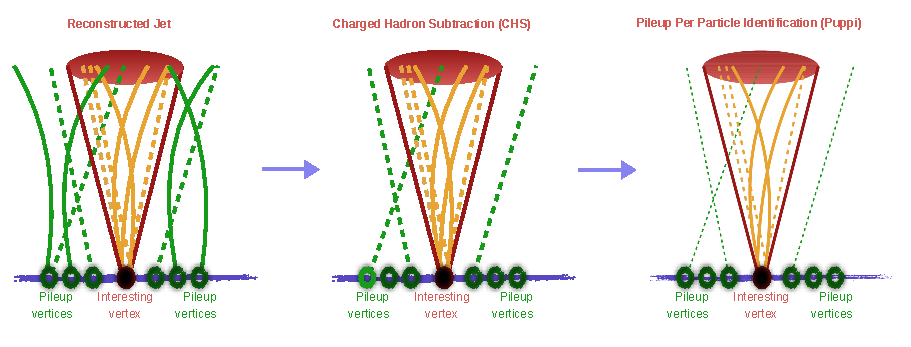
\includegraphics[width=\textwidth]{Figures/Chapter4/PU_Shematic.pdf}
\caption[Sketch of pileup suppression techniques]{
Sketch of PU suppression techniques. Solid lines correspond to charged PF candidates, while dashed lines indicate neutral PF candidates. The assigned per-particle weights (from PUPPI) are illustrated by thinner lines. Figure taken from Ref.~\cite{Jet_Reconstruction_Run2_Run3}.}
\label{Figure:Chapter4_Pileup_Schematic}
\end{figure}

To suppress misidentified jets arising from non-hadronic or spurious sources, a dedicated jet identification discriminator is applied. This discriminator evaluates a combination of variables, including the energy fractions carried by different categories of PF candidates (charged hadrons, neutral hadrons, and photons), as well as the charged and neutral particle multiplicities associated with each jet~\cite{Jet_Algorithm_Performance}. In addition, to prevent double-counting of physics objects, jets that spatially overlap with identified $\PGt$ lepton candidates are removed from the collection. Specifically, any jet falling within a cone of $\Delta R < 0.5$ around a selected $\PGt$ candidate is assumed to correspond to the same physical object and is excluded from further analysis.

\subsubsection{Bottom-quark initiated jets}

Jets originating from bottom quarks can be identified using a technique known as \textit{b-tagging}, which exploits the distinctive properties of $b$-hadron decays. A key characteristic of $b$ hadrons is their relatively long lifetime (approximately $1.5\unit{ps}$~\cite{ParticleMasses}), which allows them to travel several millimetres from the PV before decaying. Consequently, the resulting decay products are displaced from the PV and typically leave tracks that can be traced back to a \textbf{\ac{SV}}. The displacement of these tracks is quantified using the \ac{IP}, defined as the distance of closest approach of a charged particle’s trajectory to the PV. The reliability of this observable is further characterised by the \textit{IP significance}, given by the ratio of the IP to its associated uncertainty. The discriminating power of the IP in $b$-tagging is illustrated in Fig.\ref{Figure:Chapter4_IP_bjets}.

\begin{figure}[h]
\centering
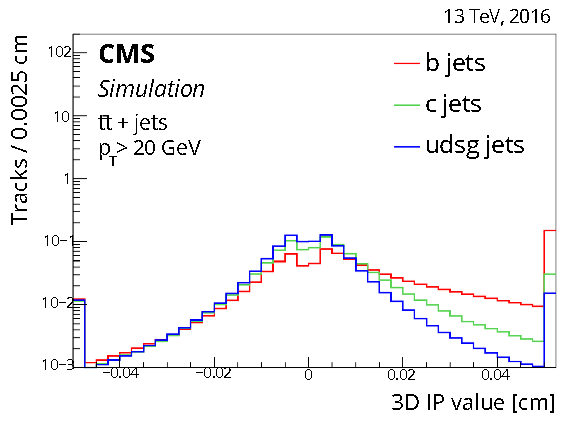
\includegraphics[width=0.7\textwidth]{Figures/Chapter4/IP_bjets.pdf}
\caption[Distributions of the 3D impact parameter for tracks associated with different types of jets]{Distributions of the 3D IP for tracks associated with different types of jets. Figure taken from Ref.~\cite{HeavyFlavourJets_ID}.}
\label{Figure:Chapter4_IP_bjets}
\end{figure}

Algorithms used to identify b-jets typically exploit lifetime-based signatures. They may also incorporate variables sensitive to other distinctive properties of b hadrons, such as their large mass and hard fragmentation behaviour. In this thesis, the employed tagger is \textbf{DeepJet}~\cite{DeepJet}, a deep neural network combining convolutional (CNN) and recurrent (LSTM) layers. DeepJet takes as input a set of global variables, PF candidate features, and SV information, and outputs class probabilities for a jet to be a b-, c-, or light-flavour jet. Its performance is summarised in Fig.~\ref{Figure:Chapter4_DeepJetPerformance}.

\begin{figure}[h]
    \centering
    % First row
    \begin{subfigure}[b]{0.49\textwidth}
        \centering
        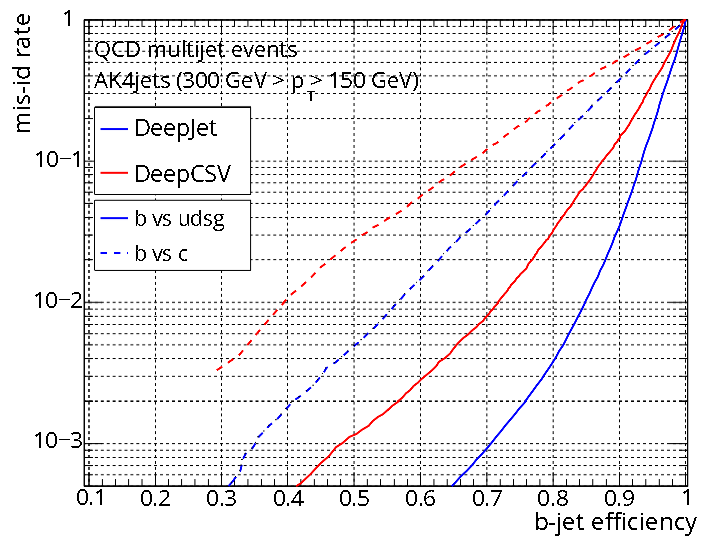
\includegraphics[width=\textwidth]{Figures/Chapter4/deepJet_lowpt.pdf}
        \caption{}
    \end{subfigure}
    \begin{subfigure}[b]{0.49\textwidth}
        \centering
        \includegraphics[width=\textwidth]{Figures/Chapter4/deepjet_mediumpt.pdf}
        \caption{}
    \end{subfigure}
\caption[Performance of the DeepJet algorithm in QCD multijet events]{Performance of the DeepJet algorithm in QCD multijet events compared to DeepCSV~\cite{HeavyFlavourJets_ID}, an alternative b-tagging algorithm. Performance is illustrated at \textbf{(a)} low jet $p_\mathrm{T}$, \textbf{(b)} medium jet $p_\mathrm{T}$. Figures taken from Ref.~\cite{DeepJet}.}

\label{Figure:Chapter4_DeepJetPerformance}
\end{figure}

\subsection{Missing transverse energy}
As mentioned in Section~\ref{Section:Chapter3_CMS_Detector_Introduction}, the total transverse momentum of a hard scattering event is assumed to be zero and is conserved. The concept and role of \textbf{MET} was also discussed, but for completeness, its definition~\cite{MET_Reconstruction} is presented here:

\begin{equation_pad}
    \vec{E}_\mathrm{T}^{\text{miss,PF}} = - \sum_i \vec{p_\mathrm{T}}^i
\end{equation_pad}

where the sum runs over all PF candidates reconstructed in the event. This definition reflects the imbalance in transverse momentum and serves as an indirect probe for particles that escape detection.

However, PF MET suffers from PU contamination, similar to PF jets, as discussed in Section~\ref{Section:Chapter4_Jets}. In addition to PU, the accuracy of $E_\mathrm{T}^{\text{miss}}$ remains sensitive to several detector-related effects: non-linear response of the calorimeter to hadrons, minimum energy thresholds in calorimeters, and track reconstruction inefficiencies. These effects are partially mitigated through the application of jet energy corrections~\cite{JetEnergyCalibration}. To further reduce the impact of PU on MET, the PUPPI algorithm is exploited, modifying $\vec{E}_\mathrm{T}^{\text{miss}}$ by weighing the $p_\mathrm{T}$ of PF candidates according to their compatibility with the PV:

\begin{equation_pad}
    \vec{E}_\mathrm{T}^{\text{miss,PUPPI}} = - \sum_i w_i\vec{p_\mathrm{T}}^i
\end{equation_pad}

\subsection{Taus}
\label{Section:Chapter4_Taus}

The reconstruction and identification of $\PGt$ leptons are fundamental to this thesis. With a mass of $m_\tau = 1.776\GeV$ and a decay length of $c\tau = 87.03\unit{\mu m}$~\cite{ParticleMasses}, the $\PGt$ lepton decays promptly before reaching the pixel tracker, and must therefore be reconstructed from its decay products. Owing to its relatively large mass, it exhibits a rich variety of decay modes, which proceed either leptonically or hadronically, as summarised in Table~\ref{Table:Chapter4_TauDecayModes}. Leptonic decays involve the $\PGt$ lepton decaying into a lighter lepton (electron or muon) and two neutrinos, while hadronic decays produce one or more charged hadrons (pions or kaons) and at least one neutrino. Leptonic $\PGt$ decays are identified using the electron and muon identification algorithms described in Sections~\ref{Section:Electron_Identification} \& \ref{Section:Muon_Identification}, respectively.

\begin{table}[htbp]
\centering
\renewcommand{\arraystretch}{1.5} % Increase row height
\arrayrulecolor{black} % Ensure outer border is black
\begin{tabular}{|c|c|c|}
\hline
Decay Mode & Resonance & Branching Fraction [\%] \\ \hline \hline 
\rowcolor{verylightblue}
Leptonic decays ($e$,$\mu$)                               & - & 35.2 \\ 
\arrayrulecolor{lightgray} \hline
$\tau^- \rightarrow e^- \overline{\nu_e} \nu_\tau$ & - & 17.8 \\ 
\arrayrulecolor{lightgray} \hline
$\tau^- \rightarrow \mu^- \overline{\nu_\mu} \nu_\tau$ & - & 17.4 \\ 
\arrayrulecolor{lightgray}  \hline 
\rowcolor{verylightblue}
Hadronic decays ($\PGt_h$)   & - & 64.8 \\ 
\arrayrulecolor{lightgray} \hline
$\tau^- \rightarrow h^- \nu_\tau$ & - & 11.5 \\ 
\arrayrulecolor{lightgray} \hline
$\tau^- \rightarrow h^- \pi^0\nu_\tau$ & $\rho(770)$ & 25.9 \\ 
\arrayrulecolor{lightgray} \hline
$\tau^- \rightarrow h^- \pi^0\pi^0\nu_\tau$ & $\mathrm{a_1}(1260)$ & 9.5 \\ 
\arrayrulecolor{lightgray} \hline
$\tau^- \rightarrow h^- h^+ h^- \nu_\tau$ & $\mathrm{a_1}(1260)$ & 9.8 \\ 
\arrayrulecolor{lightgray} \hline
$\tau^- \rightarrow h^- h^+ h^- \pi^0\nu_\tau$ & - & 4.8 \\ 
\arrayrulecolor{lightgray} \hline
Other & - & 3.3 \\ 
\arrayrulecolor{lightgray} \hline
\arrayrulecolor{black} \hline
\end{tabular}
\caption[Dominant $\PGt$ lepton decay modes and branching fractions]{Summary of the dominant decay modes of the $\PGt$ lepton and their branching fractions. The symbol $h^\pm$ denotes a charged hadron, which is typically a charged pion ($\pi^\pm$) and less frequently a charged kaon ($K^\pm$). Values extracted from Ref.~\cite{ParticleMasses}.}
\label{Table:Chapter4_TauDecayModes}
\end{table}

To reconstruct $\PGt_h$ candidates, the \textbf{\ac{HPS}} algorithm~\cite{Tau_Reco_ID_2015,Tau_Reco_ID_2018} is employed. The reconstruction begins by identifying seed regions based on PF jets clustered using the anti-$k_T$ algorithm with a distance parameter of $R = 0.4$. All PF candidates within a cone of $\Delta R < 0.5$ around the jet axis are considered, with charged hadrons required to have $p_\mathrm{T} > 0.5\GeV$ and must be compatible with originating from the PV of the event. The second step of the HPS algorithm, known as \textit{dynamic strip reconstruction}, focuses on clustering photon and electron constituents of the jet into $\Delta\eta \times \Delta\phi$ strips. These strips are used to collect energy depositions in the ECAL associated with neutral pions produced in $\PGt_h$ decays. Initially, a fixed strip size was used in the reconstruction; however, this method proved inadequate for containing all secondary particles from the $\PGt_h$ decay in some cases. For example, nuclear interactions of charged pions in the tracker material can produce low-$p_\mathrm{T}$ secondaries outside the strip, and photon conversions can lead to displaced $e^+e^-$ pairs due to scattering and bremsstrahlung. In such cases, the isolation of a $\PGt_h$ candidate would be affected. To address this, the strip size is now dynamically adjusted~\cite{Tau_Reco_ID_2018}, and the strip clustering procedure is implemented through the following steps:

\begin{enumerate}
    \item A new strip is seeded using the electron or photon ($e/\gamma$) with the highest $p_\mathrm{T}$ that has not yet been assigned to any existing strip.
    \item The electron or photon candidate with the second-highest $p_\mathrm{T}$ is merged into the strip if it lies within,
    \begin{equation_pad}
    \begin{aligned}
        \Delta \eta &= f\left(p_\mathrm{T}^{e/\gamma}\right) + f\left(p_\mathrm{T}^\text{strip}\right) \quad,\quad \Delta \eta\left[0.05,0.15\right] \\
        \Delta \phi &= g\left(p_\mathrm{T}^{e/\gamma}\right) + g\left(p_\mathrm{T}^\text{strip}\right) \quad,\quad \Delta \phi\left[0.05,0.30\right]    
    \end{aligned}
    \end{equation_pad}
    where the functions $f$ and $g$ are defined as $f(p_\mathrm{T}) = 0.20\,p_\mathrm{T}^{-0.66}$ and $g(p_\mathrm{T}) = 0.35\,p_\mathrm{T}^{-0.71}$, with $p_\mathrm{T}$ in GeV. These values were determined from simulation, such that 95\% of electrons and photons from $\PGt_h$ decays are contained within one strip. The corresponding envelope fits are illustrated in Fig.~\ref{Figure:Chapter4_StripSizeParametrisation}.
    \item The strip position is recalculated as a $p_\mathrm{T}$-weighted average of all $e/\gamma$ strip constituents.
    \begin{equation_pad}
    \begin{aligned}
        \eta_{\text{strip}} &= \frac{\sum p_\mathrm{T}^{e/\gamma} \eta_{e/\gamma}}{p_\mathrm{T}^{\text{strip}}} ,\\
        \phi_{\text{strip}} &= \frac{\sum p_\mathrm{T}^{e/\gamma} \phi_{e/\gamma}}{p_\mathrm{T}^{\text{strip}}}
    \end{aligned}
    \end{equation_pad}
    \item The strip construction ends when no further $e/\gamma$ candidates are found within the strip window.
\end{enumerate}

\begin{figure}[h]
        \centering
        % First row
        \begin{subfigure}[b]{0.49\textwidth}
            \centering
            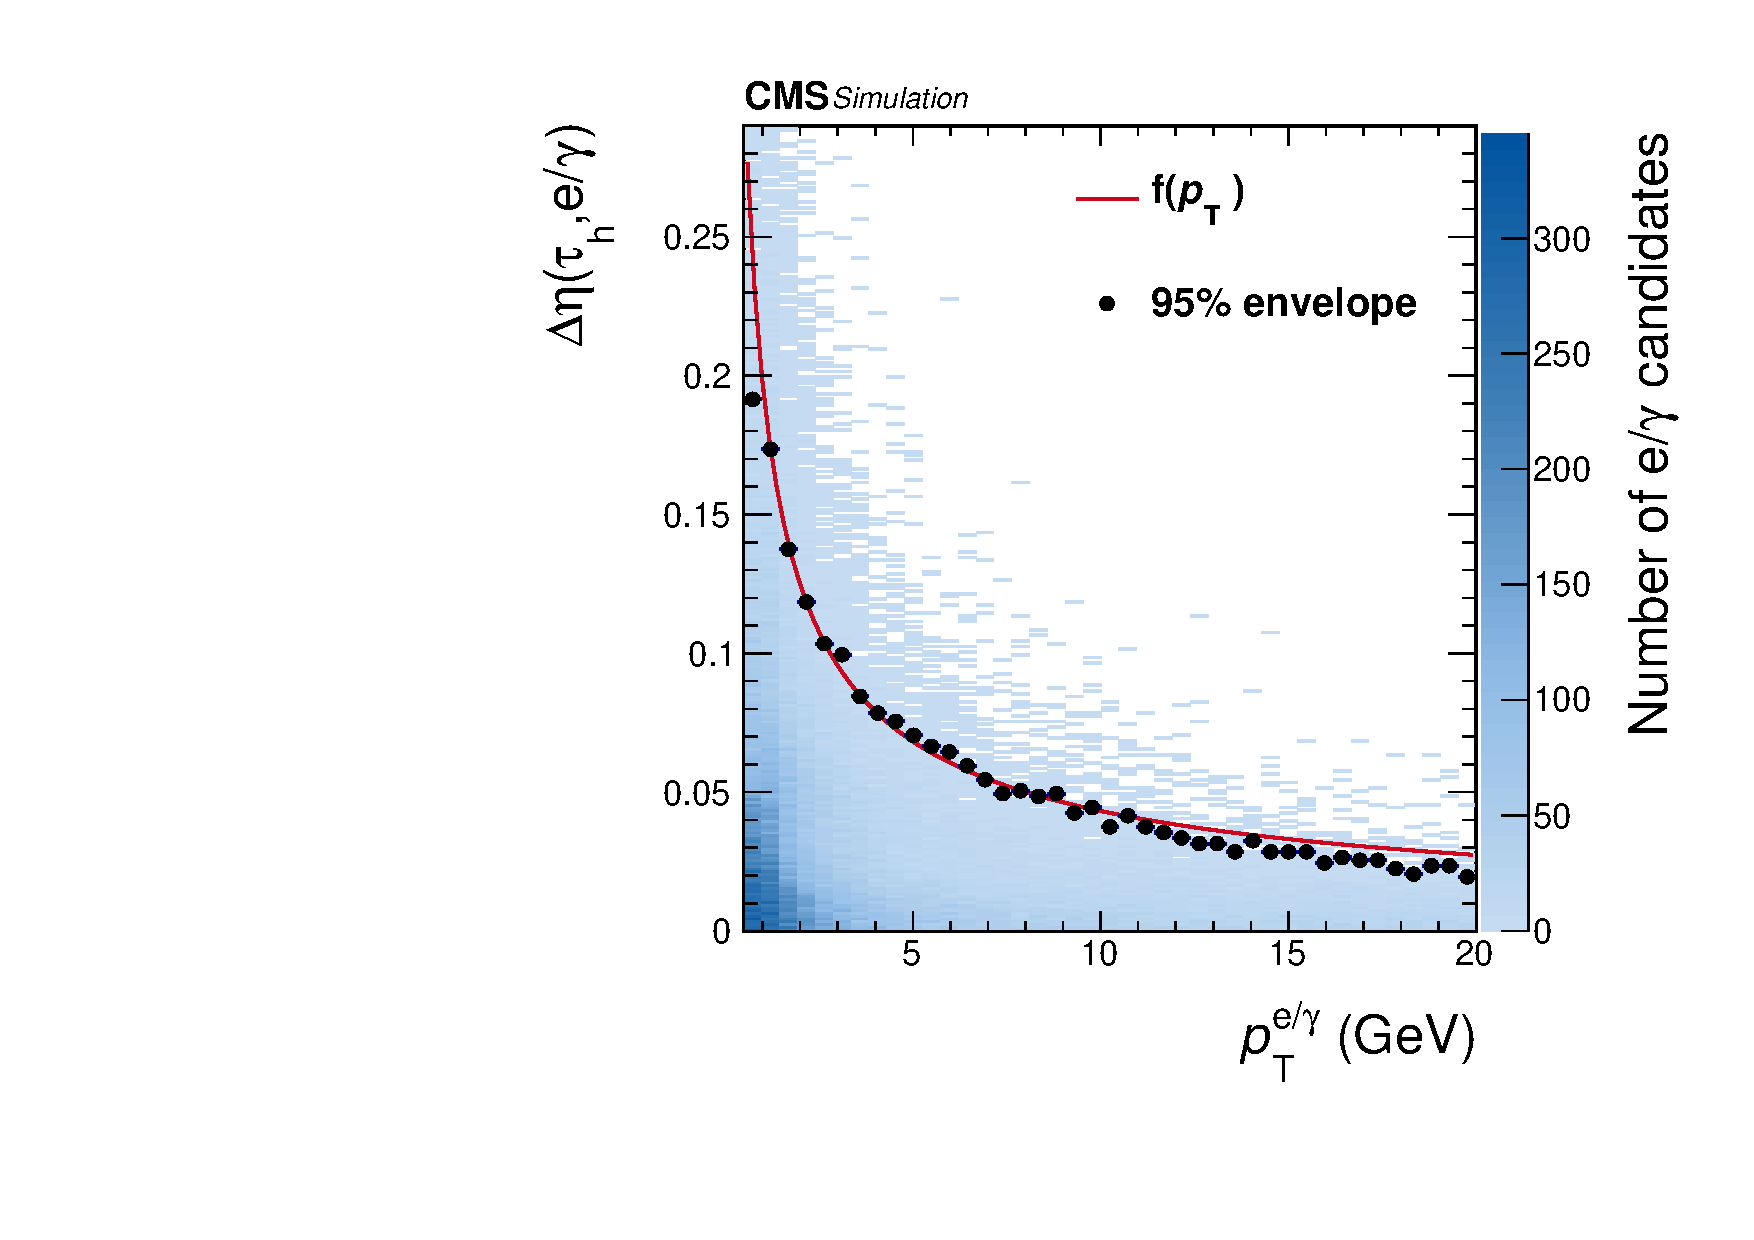
\includegraphics[width=\textwidth]{Figures/Chapter4/HPS_Envolope_Deta.pdf}
            \caption{}
        \end{subfigure}
        \begin{subfigure}[b]{0.49\textwidth}
            \centering
            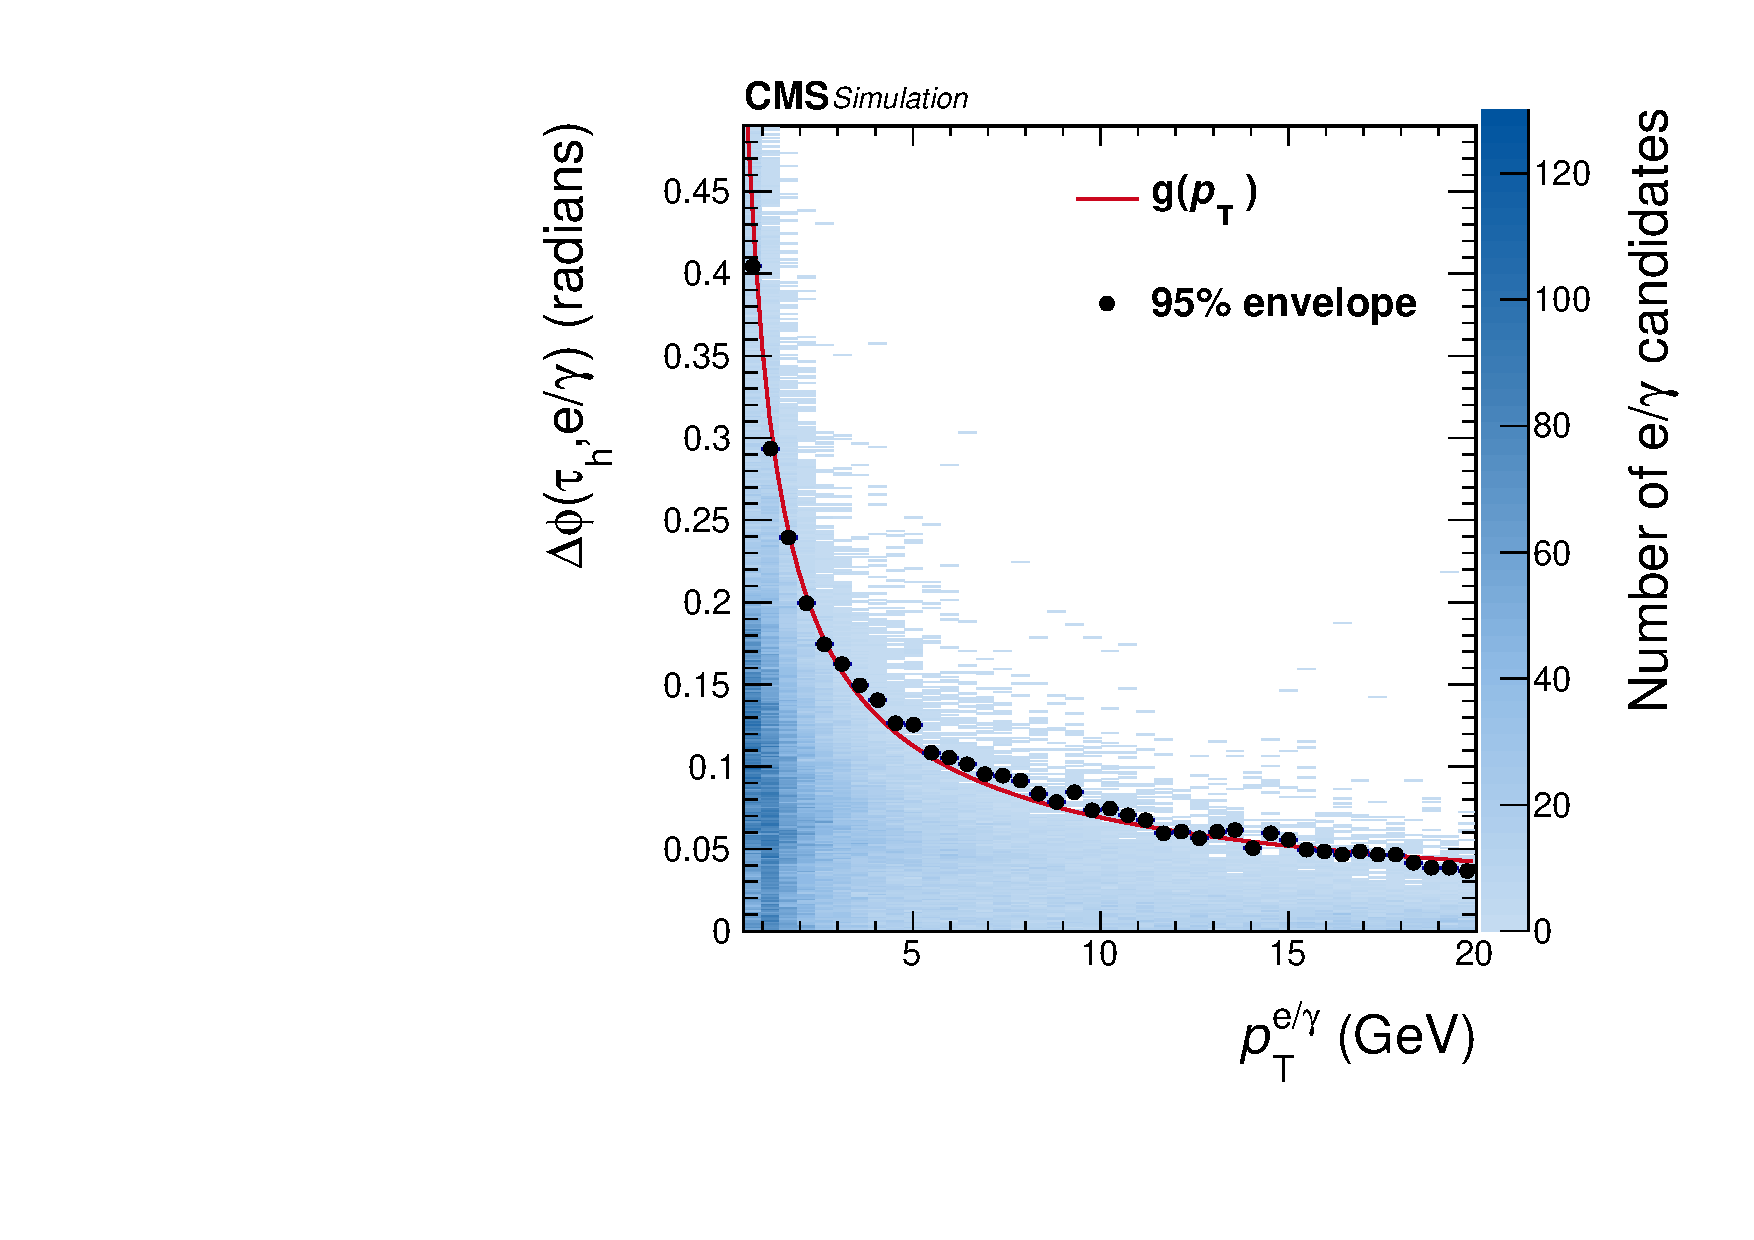
\includegraphics[width=\textwidth]{Figures/Chapter4/HPS_Envolope_Dphi.pdf}
            \caption{}
        \end{subfigure}
    \caption[Distance between $\PGt_h$ and $e/\gamma$ candidates in $\eta$ and $\phi$ coordinates as a function of the $e/\gamma$ $p_\mathrm{T}$ in simulated $\PGt_h$ decays]{Distance between $\PGt_h$ and $e/\gamma$ candidates in \textbf{(a)} $\eta$ and \textbf{(b)} $\phi$ coordinates as a function of the $e/\gamma$ $p_\mathrm{T}$ in simulated $\PGt_h$ decays. Black dots show 95\% containment boundaries, with red lines showing the corresponding fitted functions ($f,g$). Figures taken from Ref.~\cite{Tau_Reco_ID_2018}.}
    \label{Figure:Chapter4_StripSizeParametrisation}
\end{figure}

Once strips are reconstructed, they are combined with charged hadrons to form $\PGt_h$ decay mode hypotheses. The compatibility of each hypothesis is assessed by requiring the invariant mass of the visible decay products ($m_{\PGt_h}$) to lie within a predefined window tailored to each decay mode. The mass windows are optimised to maximise the reconstruction efficiency while minimising the probability of misidentifying jets as $\PGt_h$ decays. Each $\PGt_h$ decay mode is reconstructed according to the following criteria:

\begin{itemize}
    \item \textbf{$h^\pm$}: Single charged hadron with no strips. The mass window is $0 < m_{\PGt_h} < 1\GeV$, and the mass is fixed to the charged pion mass.
    \item \textbf{$h^\pm \pi^0$}: One charged hadron and one strip. The mass window is $0.3\GeV - \Delta m_{\PGt_h} < m_{\PGt_h} < 1.3\GeV\sqrt{p_\mathrm{T}^{\PGt_h}/(100\GeV)} + \Delta m_{\PGt_h}$, corresponding to the $\rho(770)$ resonance. The mass window is constrained to lie between 1.3 and 4.2$\GeV$.
    \item \textbf{$h^\pm \pi^0 \pi^0$}: One charged hadron and two strips. The mass window is $0.4\GeV - \Delta m_{\PGt_h} < m_{\PGt_h} < 1.2\GeV\sqrt{p_\mathrm{T}^{\PGt_h}/(100\GeV)} + \Delta m_{\PGt_h}$, corresponding to the $\mathrm{a}_1(1260)$. The mass window is constrained to lie between 1.2 and 4.0$\GeV$.
    \item \textbf{$h^\pm h^\mp h^\pm$}: Three charged hadrons, no strips. The mass window is $0.8 < m_{\PGt_h} < 1.5\GeV$, targeting the $\mathrm{a}_1(1260)$ resonance.
    \item \textbf{$h^\pm h^\mp h^\pm \pi^0$}: Three charged hadrons and one strip. The mass window is $0.9\GeV - \Delta m_{\PGt_h}< m_{\PGt_h} < 1.6\GeV + \Delta m_{\PGt_h}$, corresponding to the $\rho(1450)$ resonance.
\end{itemize}

The performance of the HPS algorithm in correctly identifying these decay modes is illustrated in Fig.~\ref{Figure:Chapter4_HPS_ConfusionMatrix}, which presents a confusion matrix derived from simulated $Z \rightarrow \PGt^+ \PGt^-$ events. 

\begin{figure}[h]
\centering
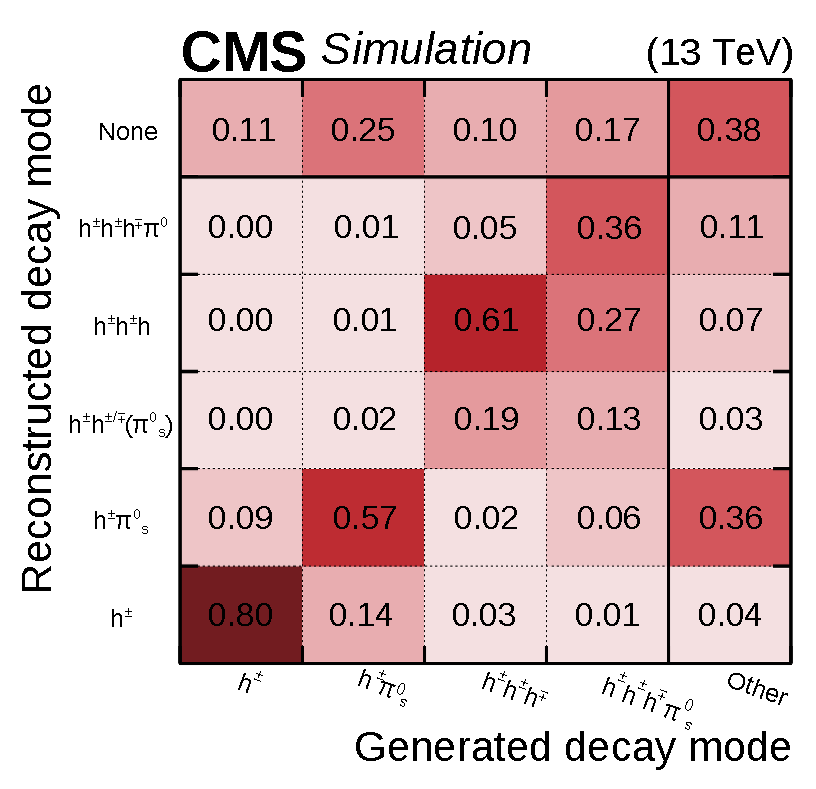
\includegraphics[width=0.6\textwidth]{Figures/Chapter4/HPS_DecayMode_Performance.pdf}
\caption[Hadronic tau decay mode confusion matrix]{Confusion matrix of reconstructed and generated $\PGt_h$ decay modes in simulation. Each cell indicates the fraction of generated decay modes reconstructed as a given decay mode. Figure extracted from Ref.~\cite{DeepTau_20-001}.}
\label{Figure:Chapter4_HPS_ConfusionMatrix}
\end{figure}

While the HPS algorithm is essential for reconstructing the decay products of $\PGt_h$ candidates and assigning decay modes, it is not sufficient on its own to effectively discriminate genuine $\PGt_h$ decays from the dominant background of quark- and gluon-initiated jets. Similarly, electrons and muons can form well-isolated single-track jets mimicking the $h^\pm$ signature, while electrons can be further misidentified as the $h^\pm \pi^0$ decay mode due to bremsstrahlung-induced ECAL clusters mimicking the photon signatures of neutral pion decays. To enhance the discrimination power and address these challenges, CMS employs a dedicated identification algorithm known as \textbf{DeepTau}~\cite{DeepTau_20-001,DeepTau_24-001}, which attempts to learn whether the input object is $\tau_h$ decay, an electron, a muon or a jet. 

DeepTau is a multiclass neural network combining convolutional and dense layers. The convolutional part of the network is designed to capture complex spatial patterns in the $\eta$–$\phi$ plane, using low-level inputs from particles surrounding the HPS candidate. These include kinematic properties, track quality, vertex compatibility (with the PV or a possible SV), calorimetric energy deposits, and pileup likelihoods. In addition to particle-level inputs, DeepTau incorporates high-level features derived from the HPS candidate, including its four-momentum, charge, decay mode, isolation variables, impact parameters, $\eta$, strip geometry, and event-level quantities such as pileup density. The output of DeepTau consists of four scores $y_\alpha$, where \textbf{[$\alpha \in {\PGt_h,\text{jet},\mu,\text{e}}$]}, each representing the estimated probability that a given $\PGt_h$ candidate belongs to class $\alpha$. From these scores, three discriminators are constructed,

\begin{equation_pad}
    D_\alpha(y) = \frac{y_{\PGt_h}}{y_{\PGt_h} + y_\alpha} 
\end{equation_pad}

which efficiently reject misidentified electrons ($D_\text{e}$), muons ($D_\mu$), and jets ($D_\text{jet}$). To support consistent application across physics analyses, a set of predefined WPs is defined for each discriminator. These working points correspond to fixed target efficiencies for identifying genuine $\PGt_h$ decays, allowing analysts to balance background rejection against signal efficiency. The expected performance of each WP is summarised in Table~\ref{Table:Chapter4_DeepTau_WPs}.

\begin{table}[htbp]
\centering
\renewcommand{\arraystretch}{1.5} % Increase row height
\begin{tabular}{|l|c|c|c|}
\hline
Working Point & $D_{\text{jet}}$ & $D_e$ & $D_\mu$ \\
\hline \hline
VVVLoose & 98\% & 99.5\% & -- \\
\arrayrulecolor{lightgray} \hline
VVLoose  & 95\% & 99\%   & -- \\
\arrayrulecolor{lightgray} \hline
VLoose   & 90\% & 98\%   & 99.95\% \\
\arrayrulecolor{lightgray} \hline
Loose    & 80\% & 95\%   & 99.9\% \\
\arrayrulecolor{lightgray} \hline
Medium   & 70\% & 90\%   & 99.8\% \\
\arrayrulecolor{lightgray} \hline
Tight    & 60\% & 80\%   & 99.5\% \\
\arrayrulecolor{lightgray} \hline
VTight   & 50\% & 70\%   & -- \\
\arrayrulecolor{lightgray} \hline
VVTight  & 40\% & 60\%   & -- \\
\arrayrulecolor{lightgray} \hline
\arrayrulecolor{black} \hline
\end{tabular}
\caption[Hadronic $\PGt$ target efficiencies for the different working points of the DeepTau algorithm with respect to the electron, muon and jet discriminators]{Hadronic $\PGt$ target efficiencies for the different WPs of the DeepTau algorithm with respect to the electron, muon and jet discriminators. Values extracted from Ref.~\cite{DeepTau_20-001}.}
\label{Table:Chapter4_DeepTau_WPs}
\end{table}

\section{Event simulation}
\label{Section:Chapter4_EventSimulation}
Simulated samples are an essential component of any analysis, enabling the modelling of both signal and background processes. Therefore, a brief overview of the event generation procedure is warranted. \ac{MC} simulators are employed to model pp collisions according to theoretical predictions, ensuring that events are sampled with the appropriate level of randomness to reflect the underlying probability distributions of the physical processes involved~\cite{PYTHIA,EventGenerators}.

The simulation of pp collisions proceeds through several distinct steps, each modelling a different stage of the event:

\begin{enumerate}
    \item \textbf{Hard scattering process:} The hard scattering process is generated using perturbative matrix-element calculations, corresponding to high-energy interactions at short distance scales where QCD remains asymptotically free. This step models the distribution of initial-state partons within the proton via \acp{PDF}, and computes the relevant matrix element, $\mathcal{M}_{i \to f}$, for a given set of model parameters $\vec{\alpha}$. Parton-level final states are then produced with probabilities proportional to the squared matrix element.

    \item \textbf{Parton showers:} In this step, \textit{\ac{ISR}} and \textit{\ac{FSR}} are simulated. This models the emission of coloured partons that can occur before or after the hard scattering process.

    \item \textbf{Hadronisation:} At low energy scales, QCD enters the non-perturbative regime, where the coloured partons from the parton shower combine to form colour-neutral hadrons. This step is modelled using QCD phenomenological models with tunable parameters that are adjusted to match experimental data.

    \item \textbf{Particle decays:} Unstable particles produced in the event are decayed according to their lifetimes and branching fractions, resulting in stable final-state particles.

    \item \textbf{Underlying event:} Additional softer interactions between the remaining proton constituents (spectator partons) are simulated, contributing further particles to the event.

    \item \textbf{Detector simulation:} The final step models the passage of particles through the CMS detector using a detailed simulation of its geometry and material composition.
\end{enumerate}


% The main background processes (excluding W+jets and DY) and the corresponding simulation details are summarised below:
% \begin{itemize}
%     \item \textbf{W+jets}: Simulated at LO using $\MADGRAPH$~\cite{MadGraph}.
%     \item \textbf{Triboson ($\PW\PW\PW$, $\PW\PW\PZ$, $\PW\PZ\PZ$, $\PZ\PZ\PZ$)}: Simulated at NLO using \\ $\MGvATNLO$~\cite{MadGraph}.
%     \item \textbf{$\ttbar$}: Simulated at NLO accuracy using $\POWHEG$ 2.0~\cite{Powheg_1,Powheg_2,Powheg_3}. Top quark pairs primarily decay via $t\overline{t} \to b \overline{b} \PW^+ \PW^-$, resulting in final states that may include genuine leptons as well as jets that can be misidentified as $\PGt_h$ candidates.
%     \item \textbf{Diboson ($\PW\PW$, $\PW\PZ$, $\PZ\PZ$)}: Simulated at NLO accuracy with \\ $\MGvATNLO$~\cite{MadGraph}. 
%     \item \textbf{Triboson ($\PW\PW\PW$, $\PW\PW\PZ$, $\PW\PZ\PZ$, $\PZ\PZ\PZ$)}: Simulated at NLO using \\ $\MGvATNLO$~\cite{MadGraph}.
%     \item \textbf{Single top}: Includes $t$-channel and $tW$ production, simulated at NLO with \\ 
%     $\POWHEG$ 1.0~\cite{Powheg_0}.
%     \item \textbf{Electroweak $\PW$ and $\PZ$}: Simulated at LO with $\MADGRAPH$~\cite{MadGraph}.
% \end{itemize}